\documentclass[border=10pt]{standalone}
\usepackage{amsmath}
\usepackage{tikz}
\usetikzlibrary{arrows.meta, fit, backgrounds, positioning, calc}

\definecolor{inputcol}{HTML}{4FC3F7}    % light blue — inputs
\definecolor{hiddencol}{HTML}{AB47BC}   % purple — hidden/processing layers
\definecolor{outputcol}{HTML}{66BB6A}   % green — outputs (positive pairs)
\definecolor{attncol}{HTML}{FFA726}     % orange — attention/special

\begin{document}
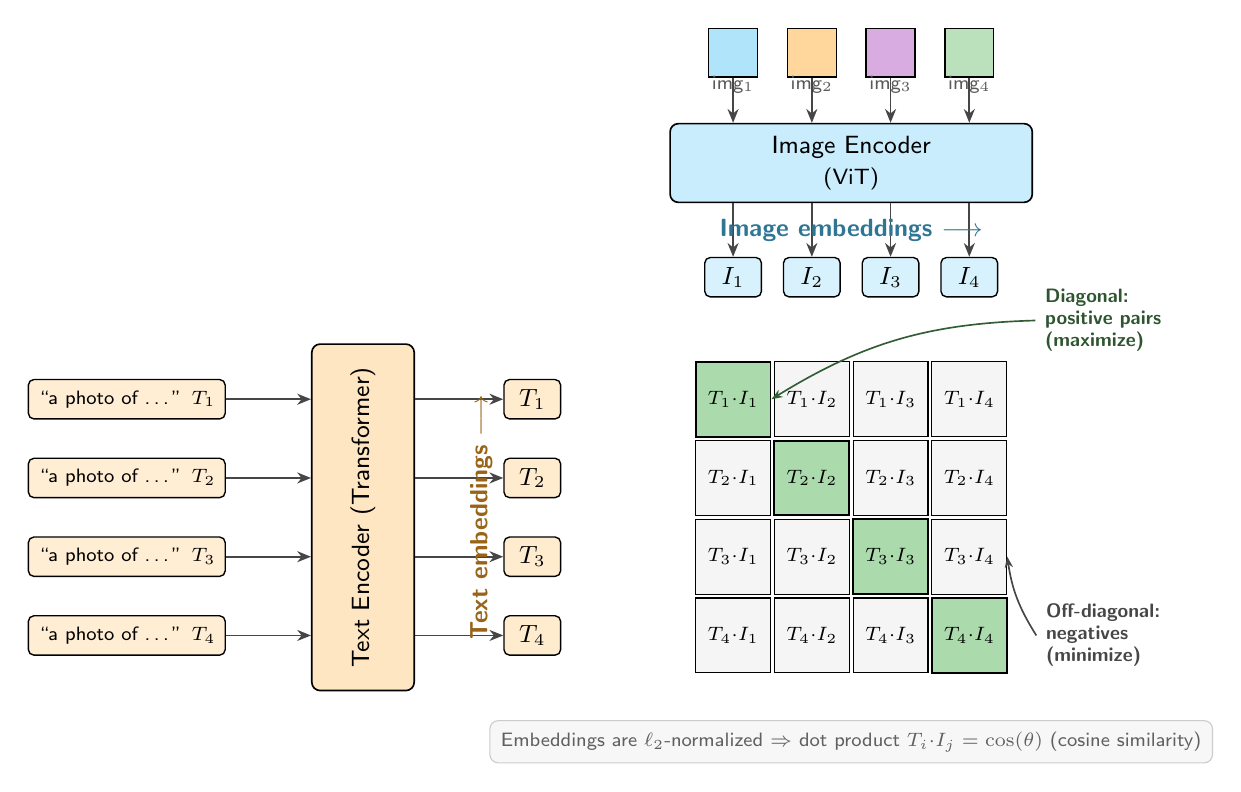
\begin{tikzpicture}[
  layer/.style={
    draw, rounded corners=3pt, minimum width=2.4cm, minimum height=1.0cm,
    font=\sffamily\small, align=center, line width=0.6pt
  },
  imgbox/.style={
    draw, minimum size=0.62cm, font=\sffamily\scriptsize, align=center,
    line width=0.5pt, inner sep=0pt
  },
  txtbox/.style={
    draw, rounded corners=2pt, minimum width=2.5cm, minimum height=0.5cm,
    font=\sffamily\scriptsize, align=center, line width=0.5pt, inner sep=2pt
  },
  emb/.style={
    draw, rounded corners=2pt, minimum width=0.72cm, minimum height=0.5cm,
    font=\sffamily\small, align=center, line width=0.5pt, inner sep=1pt
  },
  cell/.style={
    draw, minimum size=0.95cm, font=\sffamily\scriptsize, align=center,
    line width=0.4pt, inner sep=0pt
  },
  conn/.style={-{Stealth[length=5pt, width=4pt]}, line width=0.6pt, gray!55!black},
  annot/.style={font=\sffamily\scriptsize, text=gray!75!black},
]

% ---------------------------------------------------------------
% Geometry: matrix grid 4x4, cell size 0.95cm, starts at origin top-left
% Columns x = 0,1,2,3 ; Rows y = 0,-1,-2,-3  (top row = T1)
% ---------------------------------------------------------------
\def\cs{1.0}  % cell pitch

% ===== Image inputs (top-left) feeding image encoder =====
\foreach \i/\c in {1/inputcol,2/attncol,3/hiddencol,4/outputcol}{
  \node[imgbox, fill=\c!45] (im\i) at (\cs*\i + 0.0, 4.4) {};
  \node[font=\sffamily\scriptsize, text=gray!70!black] at (\cs*\i + 0.0, 4.0) {img$_\i$};
}

% Image encoder box
\node[layer, fill=inputcol!30, minimum width=4.6cm]
  (imgenc) at (\cs*2.5, 3.0) {Image Encoder\\\footnotesize (ViT)};

% Image embeddings = column headers above matrix
\foreach \j in {1,2,3,4}{
  \node[emb, fill=inputcol!22] (I\j) at (\cs*\j, 1.55) {$I_\j$};
}

% arrows: images -> encoder
\foreach \i in {1,2,3,4}{ \draw[conn] (im\i) -- (imgenc.north -| im\i); }
% encoder -> image embeddings
\foreach \j in {1,2,3,4}{ \draw[conn] (imgenc.south -| I\j) -- (I\j); }

% ===== Text inputs (left) feeding text encoder =====
\foreach \k in {1,2,3,4}{
  \pgfmathsetmacro\ty{-\cs*\k + \cs}   % aligns with matrix rows (row k at y=-(k-1)*cs)
  \node[txtbox, fill=attncol!20] (tx\k) at (-6.7, \ty) {``a photo of \ldots'' $T_\k$};
}

% Text encoder box (vertical, between text inputs and row headers)
\node[layer, fill=attncol!28, minimum height=4.4cm, minimum width=1.3cm]
  (txtenc) at (-3.7, -1.5) {\rotatebox{90}{Text Encoder (Transformer)}};

% Text embeddings = row headers to the left of matrix
\foreach \k in {1,2,3,4}{
  \pgfmathsetmacro\ty{-\cs*\k + \cs}
  \node[emb, fill=attncol!22] (T\k) at (-1.55, \ty) {$T_\k$};
}

% arrows: texts -> text encoder
\foreach \k in {1,2,3,4}{
  \pgfmathsetmacro\ty{-\cs*\k + \cs}
  \draw[conn] (tx\k) -- (txtenc.west |- tx\k);
}
% text encoder -> text embeddings
\foreach \k in {1,2,3,4}{
  \draw[conn] (txtenc.east |- T\k) -- (T\k);
}

% ===== Similarity matrix 4x4 =====
% rows = text T_i (top->bottom i=1..4), cols = image I_j (left->right j=1..4)
\foreach \i in {1,2,3,4}{
  \foreach \j in {1,2,3,4}{
    \pgfmathsetmacro\ry{-\cs*\i + \cs}
    \ifnum\i=\j
      \node[cell, fill=outputcol!55, line width=0.7pt] (m\i\j) at (\cs*\j, \ry)
        {$T_{\i}{\cdot}I_{\j}$};
    \else
      \node[cell, fill=gray!8] (m\i\j) at (\cs*\j, \ry) {$T_{\i}{\cdot}I_{\j}$};
    \fi
  }
}

% Axis labels
\node[font=\sffamily\small\bfseries, text=inputcol!60!black]
  at (\cs*2.5, 2.15) {Image embeddings $\longrightarrow$};
\node[font=\sffamily\small\bfseries, text=attncol!60!black, rotate=90]
  at (-2.2, -1.5) {Text embeddings $\longrightarrow$};

% ===== Annotations =====
% positive pairs annotation (point to diagonal)
\node[annot, text=outputcol!45!black, align=left, font=\sffamily\scriptsize\bfseries]
  (posann) at (\cs*5.7, 1.0) {Diagonal:\\positive pairs\\(maximize)};
\draw[-{Stealth[length=4pt]}, outputcol!50!black, line width=0.6pt]
  (posann.west) to[bend right=15] (m11.east);

% negatives annotation
\node[annot, text=gray!55!black, align=left, font=\sffamily\scriptsize\bfseries]
  (negann) at (\cs*5.7, -3.0) {Off-diagonal:\\negatives\\(minimize)};
\draw[-{Stealth[length=4pt]}, gray!55!black, line width=0.6pt]
  (negann.west) to[bend left=12] (m34.east);

% L2-normalization note
\node[annot, align=center, draw=gray!40, rounded corners=3pt, fill=gray!6,
      inner sep=4pt, font=\sffamily\scriptsize]
  at (\cs*2.5, -4.35)
  {Embeddings are $\ell_2$-normalized $\Rightarrow$ dot product $T_i{\cdot}I_j = \cos(\theta)$ (cosine similarity)};

\end{tikzpicture}
\end{document}
